\documentclass[]{article}

\usepackage[italian]{babel}
\usepackage[margin=20mm, footskip = 20pt]{geometry}
\usepackage{array}
\usepackage{tabularx}
\usepackage{graphicx}
\usepackage{subfiles}
\usepackage{hyperref}
\usepackage{nameref}
\usepackage{titlesec}
\usepackage{longtable}
\usepackage[table]{xcolor}
\usepackage{titling}
\usepackage{lastpage}
\usepackage{ifthen}
\usepackage{calc}
\usepackage{soulutf8}
\usepackage{contour}
\usepackage{float}
\usepackage{fancyhdr}
\usepackage{multirow}
\usepackage{pgfgantt}
\usepackage{lscape}

\newcommand{\hr}{\par\vspace{-.1\ht\strutbox}\noindent\hrulefill\par}

\graphicspath{ {./}
	{./commons/res}
}

%--------------------------------------------------
% Comandi per inserire contenuto del documento
%--------------------------------------------------
\makeatletter

\newcommand\appendToGraphicsPath[1]{%
	\g@addto@macro\Ginput@path{{#1}}%
}

\newcommand{\setTitle}[1]{%
	\newcommand{\@phTitle}{#1}%
}
\newcommand{\phTitle}{\@phTitle}

\newcommand{\setDate}[1]{%
	\newcommand{\@phDate}{#1}%
}
\newcommand{\phDate}{\@phDate}

\newcommand{\setUso}[1]{%
	\newcommand{\@uso}{#1}%
}
\newcommand{\uso}{\@uso}

\newcommand{\setVersione}[1]{%
	\newcommand{\@versione}{#1}%
}
\newcommand{\versione}{\@versione}

\newcommand{\disabilitaVersione}{%
	\renewcommand{\setVersione}[1]{}%
	\renewcommand{\versione}{DISABILITATA}
}

\newcommand{\setResponsabile}[1]{%
	\newcommand{\@responsabile}{#1}%
}
\newcommand{\responsabile}{\@responsabile}

\newcommand{\setRedattori}[1]{%
	\newcommand{\@redattori}{#1}%
}
\newcommand{\redattori}{\@redattori}

\newcommand{\setVerificatori}[1]{%
	\newcommand{\@verificatori}{#1}%
}
\newcommand{\verificatori}{\@verificatori}

\newcommand{\setModifiche}[1]{%
	\newcommand{\@modifiche}{#1}%
}
\newcommand{\modifiche}{\@modifiche}

\makeatother 

%--------------------------------------------------
% Comandi per i documenti esterni e il glossario
%--------------------------------------------------

\newcommand{\dext}[1]{\textsc{#1\textsubscript{\textit{D}}}}

\newcommand{\glock}[1]{\textsc{#1\textsubscript{\textit{G}}}}

%--------------------------------------------------
% Comandi per impostare sottotitoli di quarto e quinto livello
%--------------------------------------------------

\setcounter{secnumdepth}{4}
\setcounter{tocdepth}{4}

\titleformat{\paragraph}
{\normalfont\normalsize\bfseries}{\theparagraph}{1em}{}
\titlespacing*{\paragraph}{0pt}{2.25ex plus 1ex minus .2ex}{1.5ex plus .2ex}

\titleformat{\subparagraph}
{\normalfont\normalsize\bfseries}{\thesubparagraph}{1em}{}
\titlespacing*{\subparagraph}{0pt}{1.75ex plus 1ex minus .2ex}{.75ex plus .1ex}

\appendToGraphicsPath{../../commons/res/}

%------------------------------
%
% COMANDI DI CONFIGURAZIONE
%
%------------------------------

\setTitle{Analisi dei Requisiti}

\setVersione{2.0.0}

\setDate{14-03-2021}

\setResponsabile{Lucia Fenu}

\setRedattori{
    Alessandro Chimetto\\&
    Alessandro Dindinelli\\&
    Giacomo Bulbarelli\\&
    Valton Tahiraj
}

\setVerificatori{
	Giacomo Bulbarelli\\&
    Alessandro Chimetto\\&
	Alessandro Dindinelli\\&
	Lucia Fenu\\&
	Valton Tahiraj
}

\setUso{Esterno}

\setModifiche{
	2.0.0 & Lucia Fenu & Responsabile & 14-03-2021 & Approvazione documento \\
    1.3.0 & Alessandro Chimetto & Verificatore & 14-03-2021 & Verifica numerazione casi d'uso \\
	1.2.0 & Valton Tahiraj   & Analista & 13-03-2021 & Modifiche numerazione casi d'uso \\
	1.2.0 & Giacomo Bulbarelli    & Verificatore & 13-03-2021 & Verifica revisione casi d'uso \\
    1.1.0 & Alessandro Dindinelli & Analista & 13-03-2021 & Revisionati casi d'uso \\
    1.1.0 & Alessandro Chimetto & Verificatore & 12-03-2021 & Verifica sezione 2.2.1 e modifiche ai requisiti\\
	1.0.0 & Giacomo Bulbarelli	& Amministratore & 12-03-2021 & Aggiunta sezione 2.2.1 "Mappatura dell'ambiente" e modifica dei requisiti di vincolo \\
	1.0.0 & Valton Tahiraj   & Responsabile & 09-01-2021 & Approvazione documento \\
	0.9.0 & Lucia Fenu   & Verificatore & 08-01-2021 & Correzioni generali \\
	0.9.0 & Valton Tahiraj   & Verificatore & 08-01-2021 & Verifica aggiunta introduzione\\
    0.8.0 & Alessandro Chimetto & Analista & 08-01-2021 & Aggiunta introduzione\\
	0.8.0 & Lucia Fenu	& Verificatore & 08-01-2021 & Verificato descrizione generale \\
    0.7.0 & Alessandro Chimetto & Analista & 08-01-2021 & Aggiunta descrizione generale\\
	0.7.0 & Alessandro Dindinelli & Verificatore & 08-01-2021 & Verifica tabelle fonte-requisiti e requisito-fonti\\
	0.6.0 & Valton Tahiraj & Analista & 07-01-2021 & Stesura tabelle fonte-requisiti e requisito-fonti\\
	0.6.0 & Valton Tahiraj   & Verificatore & 07-01-2021 & Verifica aggiunta tabella requisiti \\
	0.5.0 & Alessandro Dindinelli & Analista& 07-01-2021 & Aggiunta tabella requisiti \\
    0.5.0 & Giacomo Bulbarelli & Verificatore & 07-01-2021 & Verificato UC5 \\
    0.4.1 & Alessandro Chimetto & Analista & 06-01-2021 & Aggiunta analisi di UC5: Controllo unità\\
	0.4.1 & Valton Tahiraj        & Verificatore   & 06-01-2021 & Verifica suddivisione UC6 \\
	0.4.0 & Alessandro Dindinelli & Analista & 06-01-2021 & Modifica suddivisione UC6\\
    0.4.0 & Alessandro Chimetto & Verificatore & 06-01-2021 & Verificati UC1, UC4 e attori\\
	0.3.0 & Giacomo Bulbarelli & Analista & 05-01-2021 & Inserito diagramma e descrizione degli attori\\
	0.3.0 & Giacomo Bulbarelli & Analista & 05-01-2021 & Inserito UC relativo alla mappatura\\
	0.3.0 & Giacomo Bulbarelli & Analista & 05-01-2021 & Inserito UC relativo alla guida introduttiva \\
	0.3.0 & Alessandro Dindinelli & Verificatore & 05-01-2021 & Verificato introduzione requisiti e tabella requisiti \\
	0.2.1 & Valton Tahiraj & Analista & 05-01-2021 & Stesura introduzione requisiti e tabella requisiti \\
    0.2.1 & Alessandro Chimetto & Verificatore & 05-01-2021 & Verificato UC6.1.7\\
	0.2.0 & Alessandro Dindinelli & Analista & 05-01-2021 & Aggiunto UC6.1.7\\
	0.2.0 & Valton Tahiraj        & Verificatore   & 04-01-2021 & Verifica stesura UC6 amministrazione\\
	0.1.0 & Alessandro Dindinelli & Analista & 04-01-2021 & Stesura UC6 amministrazione\\
	0.1.0 & Alessandro Dindinelli & Verificatore & 04-01-2021 & Verificati UC2 e UC3\\
    0.0.2 & Valton Tahiraj & Analista & 03-01-2021 & Stesura UC2 login e UC3 logout\\
	0.0.2 & Valton Tahiraj & Verificatore & 03-01-2021 & Verifica modifica struttura documento\\
    0.0.1 & Alessandro Chimetto & Analista & 03-01-2021 & Modifica struttura documento\\
    0.0.1 & Giacomo Bulbarelli & Verificatore & 31-12-2020 & Verificata prima stesura\\
	0.0.0 & Valton Tahiraj & Analista & 31-12-2020 & Prima stesura
}

\begin{document}

	% Direttive per la creazione del titolo tramite comando maketitle
\title{\huge \textsc{\phTitle{}} \\
	\vspace{11pt} \large \textsc{\phDate{}}}

\author{} % Non toccare
\date{} % Non toccare

%--------------------
% Frontespizio
%--------------------

% Logo del gruppo
\begin{figure}[t!]
	\centering
	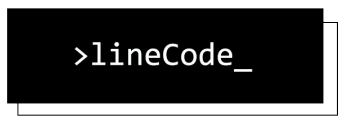
\includegraphics[width=20em]{lclong}
\end{figure}

% Titolo / Nome
\maketitle
\thispagestyle{empty}

% Dati specifici sul doc in forma tabulare
\begin{table}[ht]
	\begin{center}
		\label{tab:Dati sul documento}
		\begin{tabular}{r|l}
			\multicolumn{2}{c}{ \textsc{Dati sul documento} } \\
			\hline
			\textbf{Versione} & \versione{} \\
			\textbf{Uso} & \uso{}  \\
			\textbf{Redattori} & \redattori{} \\
			\textbf{Verificatori} & \verificatori{} \\
			\textbf{Responsabile} & \responsabile{} \\
			\textbf{Destinatari} & lineCode \\
								& prof.\ Vardanega Tullio \\		
								& prof.\ Cardin Riccardo \\
			\ifthenelse{\equal{\uso}{Esterno}}{
								& Sanmarco Informatica
			}{} \\
		\end{tabular}
	\end{center}
\end{table}

\newpage

\renewcommand{\arraystretch}{2} % allarga le righe con dello spazio sotto e sopra
\begin{longtable}[H]{>{\centering\bfseries}m{2cm} >{\centering}m{3.5cm} >{\centering}m{2.5cm} >{\centering}m{3cm} >{\centering\arraybackslash}m{5cm}}
	\rowcolor{lightgray}
	{\textbf{Versione}} & {\textbf{Nominativo}} & {\textbf{Ruolo}} & {\textbf{Data}} & {\textbf{Descrizione}}  \\
	\endfirsthead%
	\rowcolor{lightgray}
	{\textbf{Versione}} & {\textbf{Nominativo}}  & {\textbf{Ruolo}} & {\textbf{Data}} & {\textbf{Descrizione}}  \\
	\endhead%
	\modifiche{}%
\end{longtable}
	\newpage

    \tableofcontents
    \listoffigures
    \listoftables
    \newpage

	%--------------------------------
	%
	% IL CONTENUTO INIZIA DA QUI
	%
	%--------------------------------

	\section{Introduzione}
	\subsection{Scopo del documento}
Il documento ha lo scopo di definire le guidelines del way of working adottato dal team lineCode. Le attività presenti in questo documento sono redatte da processi contenuti nello standard ISO/IEC 12207:1995. Risulta quindi necessario che tutti i membri del gruppo prendano visione di questo documento ai fini di coesione e uniformità all'interno del progetto.

\subsection{Scopo del prodotto}
Il \glock{capitolato} C5 ha come obbiettivo la realizzazione di un applicativo \glock{Real-Time} in grado di guidare delle unità dotate di mobilità autonoma in ambienti specifici, partendo dal presupposto che queste si muovano in ambienti in cui sono presenti altre unità (autonome o meno).

\subsection{Glossario e documenti esterni}
In supporto alla documentazione viene fornito un glossario per chiarire, con una definizione, eventuali termini specifici contenuti in questo documento.
Saranno adottati quindi questi due simboli a pedice:
\begin{itemize}
	\item \textit{D} se indicano un documento specifico;
	\item \textit{G} se incluse nel \dext{glossario}.
\end{itemize}

\subsection{Riferimenti}
	\subsubsection{Riferimenti normativi}
	\begin{itemize}
		\item \textbf{{C5 - PORTACS}}: \url{https://www.math.unipd.it/~tullio/IS-1/2020/Progetto/C5.pdf};
        \item \textbf{Oracle Java Code Conventions}: \url{https://www.oracle.com/technetwork/java/codeconventions-150003.pdf};
        \item \textbf{Angular coding style guide}: \url{https://angular.io/guide/styleguide}.
	\end{itemize}
	\subsubsection{Riferimenti informativi}
	\begin{itemize}
		\item \textbf{ISO/IEC 12207:1995}: \url{https://www.math.unipd.it/~tullio/IS-1/2009/Approfondimenti/ISO_12207-1995.pdf};
		\item \textbf{Gitflow}: \url{http://nvie.com/posts/a-successful-git-branching-model/};
		\item \textbf{Documentazione Zapier}: \url{https://zapier.com/help};
		\item \textbf{Documentazione act}: \url{https://github.com/nektos/act/blob/master/README.md};
		\item \textbf{Studio di Fattibilità}: \dext{Studio di Fattibilità v1.0.0};
		\item \textbf{Piano di Qualifica}: \dext{Piano di Qualifica v2.0.0};
		\item \textbf{Piano di Progetto}: \dext{Piano di Progetto v2.0.0}.
	\end{itemize}
	\newpage

	\section{Descrizione generale}
	\subsection{Obiettivi del prodotto}
Il progetto \textit{PORTACS} pone come obiettivo lo studio di problematiche trasversali al mondo della logistica fra cui analisi, monitoraggio, predittività e capacità decisionale in ambito \glock{real-time}. In particolare, il \glock{capitolato} enuncia una serie di contesti con punti in comune rilevanti come il movimento di veicoli a guida (semi-)autonoma che devono raggiungere dei \glock{POI} ed evitare le collisioni.
\\\\
Data la vastità del mondo della logistica, il proponente richiede che venga preso in considerazione uno specifico contesto fra quelli (o similare a quelli) proposti nella documentazione del capitolato. Su di esso, andranno tarati i requisiti in modo da garantire che il servizio sia sempre disponibile e il più possibile privo di collisioni.

\subsection{Contesto e funzioni del prodotto}
Il contesto scelto per questo progetto è quello del ristorante dotato di camerieri robot (da qui in poi ``unità").
	\subsubsection{Mappatura dell'ambiente}    
    L'ambiente in cui si muovono le unità è rappresentato da una mappatura strutturata a griglia e tale griglia viene a sua volta divisa in celle per permettere di individuare il punto in cui l'unità si trova nel locale.
    \subsubsection{Unità}
    Le unità si muovono all'interno del ristorante rappresentato dalla struttura descritta nella sezione precedente. Ogni unità svolge ciclicamente determinate operazioni:
    \begin{enumerate}
        \item l'unità si trova ferma in una base di ricarica comunicante con la cucina dove riceve il cibo da consegnare;
        \item l'operatore si autentica al sistema e inserisce, nella coda degli ordini dell'unità, tutti i \glock{POI} su cui si dovrà effettuare la consegna;
        \item l'unità, ricevuta l'autorizzazione a partire, riceve dal sistema i dati sul percorso da seguire per consegnare tutti gli ordini;
        \item terminate le consegne, l'unità torna alla base dove potrà ricevere nuovi ordini da consegnare.
    \end{enumerate}
    L'unità comunica costantemente al sistema i suoi dati, compresi quelli che riguardano la sua sensoristica interna, in modo da ricevere istruzioni su eventuali cambi di percorso.

    \subsubsection{Cliente}
    Il cliente dispone di una vista sulla mappa del ristorante e sulle unità che si muovono in essa. La sua interfaccia risulta \glock{user-friendly}, utilizzabile senza precedente formazione.

    \subsubsection{Utente autenticato}
    È un operatore che usufruisce quotidianamente del sistema (per esempio un cuoco o un caposervizio) gestendo le unità con le rispettive code degli ordini. La sua interfaccia è sufficientemente \glock{user-friendly} da poter essere utilizzata immediatamente dopo una breve spiegazione.

    \subsubsection{Amministratore}
    Gestisce la mappa del locale e l'associazione delle unità al sistema. Conosce approfonditamente il sistema.

\subsection{Macro-architetture del prodotto}
    \subsubsection{\glock{Back-end}}
    Il \glock{back-end} è composto da più server che interagiscono fra loro per garantire ridondanza ed evitare interruzioni del servizio secondo una logica di \glock{zero downtime}.

    \subsubsection{\glock{Front-end}}
    Il \glock{front-end} mette a disposizione di tutti gli utenti una mappa con le unità che si muovono in essa e delle apposite interfacce di gestione per operatori ed amministratori.
	\newpage

	\section{Casi d'uso}
	\subsection{Attori dei casi d'uso}

\newpage
\subsection{Elenco dei casi d'uso}

	\subsubsection{UC6 - Amministrazione di sistema}
	\begin{center}
		\begin{figure}[h!]
			\includegraphics[width=8cm]{images/.jpg}
			\caption{Diagramma UC6}
		\end{figure}
	\end{center}
	\begin{itemize}
		\item \textbf{Attori primari:} utente amministratore;
		\item \textbf{Descrizione:} l'amministratore intende visualizzare le componenti del sistema, ed apportare le modifiche volute;
		\item \textbf{Scenario principale:} 
			\begin{itemize}
				\item l'amministratore gestisce la lista utenti (UC6.1);
				\item l'amministratore gestisce la mappatura dell'ambiente (UC6.2);
				\item l'amministratore gestisce la lista unità (UC6.3).
			\end{itemize}
		\item \textbf{Precondizione:} l'amministratore ha accesso alle componenti del sistema;
		\item \textbf{Postcondizione:} le componenti del sistema, rispetto al loro stato iniziale, risultano modificate come voluto.
	\end{itemize}
	
\subsubsection{UC6.1 - Gestione lista utenti}
	\begin{center}
		\begin{figure}[h!]
			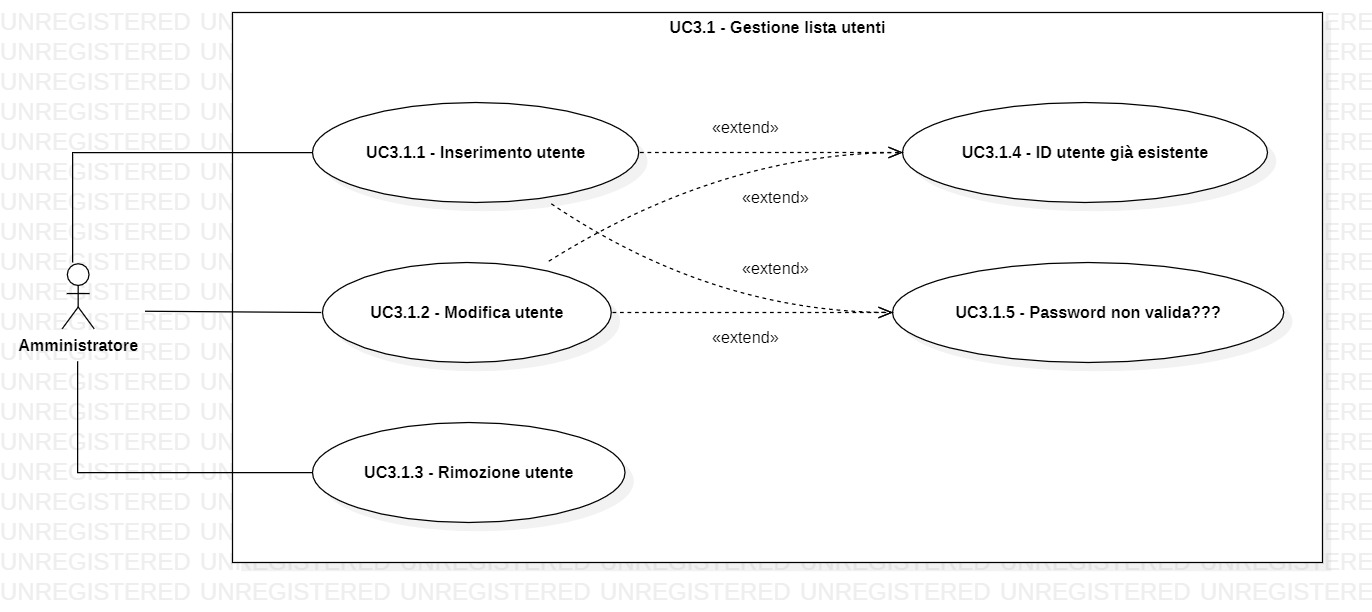
\includegraphics[width=15cm]{images/uc3.1.jpg}
			\caption{Diagramma UC6.1}
		\end{figure}
	\end{center}
	\begin{itemize}
		\item \textbf{Attori primari:} utente amministratore;
		\item \textbf{Descrizione:} l'amministratore visiona la lista degli utenti che hanno accesso al sistema, ed applica le modifiche volute;
		\item \textbf{Scenario principale:} 
			\begin{itemize}
				\item l'amministratore inserisce un utente (UC6.1.1);
				\item l'amministratore modifica un utente (UC6.1.2);
				\item l'amministratore elimina un utente (UC6.1.3).
			\end{itemize}
		\item \textbf{Precondizione:} l'amministratore visualizza l'elenco degli utenti esistenti;
		\item \textbf{Postcondizione:} la lista degli utenti, rispetto allo stato iniziale, risulta modificata come voluto.
	\end{itemize}

\subsubsection{UC6.1.1 - Inserimento utente}
\begin{itemize}
	\item \textbf{Attori primari:} utente amministratore;
	\item \textbf{Descrizione:} l'amministratore intende aggiungere un nuovo utente, alla lista degli utenti che hanno accesso al sistema;
	\item \textbf{Scenario principale:} l'amministratore inserisce le credenziali dell'utente interessato alla lista di quelli già esistenti;
	\item \textbf{Precondizione:} l'amministratore visualizza l'elenco degli utenti esistenti;
	\item \textbf{Postcondizione:} la lista degli utenti risulta aggiornata con l'aggiunta dell'utente interessato.
	\item \textbf{Estensioni:}
		\begin{itemize}
			\item \textbf{UC6.1.4:} se si tenta di usare un nome utente già esistente, viene visualizzato un apposito messaggio di errore;
			\item \textbf{UC6.1.5:} se si tenta di creare una password che non rispetta le regole di formattazione stabilite, viene visualizzato un apposito messaggio di errore.
		\end{itemize}
\end{itemize}

\subsubsection{UC6.1.2 - Modifica utente}
\begin{itemize}
	\item \textbf{Attori primari:} utente amministratore;
	\item \textbf{Descrizione:} l'amministratore intende modificare le credenziali di un utente già esistente;
	\item \textbf{Scenario principale:} l'amministratore modifica le credenziali dell'utente interessato, presente nella lista degli utenti;
	\item \textbf{Precondizione:} l'amministratore visualizza l'elenco degli utenti esistenti;
	\item \textbf{Postcondizione:} le credenziali dell'utente interessato risultano aggiornate come voluto.
	\item \textbf{Estensioni:}
	\begin{itemize}
		\item \textbf{UC6.1.4:} se si tenta di usare un nome utente già esistente, viene visualizzato un apposito messaggio di errore;
		\item \textbf{UC6.1.5:} se si tenta di creare una password che non rispetta le regole di formattazione stabilite, viene visualizzato un apposito messaggio di errore.
	\end{itemize}
\end{itemize}

\subsubsection{UC6.1.3 - Rimozione utente}
\begin{itemize}
	\item \textbf{Attori primari:} utente amministratore;
	\item \textbf{Descrizione:} l'amministratore intende eliminare utente dalla lista degli utenti che hanno accesso al sistema;
	\item \textbf{Scenario principale:} l'amministratore cancella l'utente interessato dalla lista degli utenti;
	\item \textbf{Precondizione:} l'amministratore visualizza l'elenco degli utenti esistenti;
	\item \textbf{Postcondizione:} la lista degli utenti risulta aggiornata con la rimozione dell'utente interessato.
\end{itemize}

\subsubsection{UC6.1.4 - Errore causa nome utente già esistente}
\begin{itemize}
	\item \textbf{Attori primari:} utente amministratore;
	\item \textbf{Descrizione:} l'amministratore visualizza un errore, relativo al fatto che il nome utente che ha tentato di assegnare all'utente è già in uso;
	\item \textbf{Scenario principale:} l'amministratore tenta di inserire un nome utente non valido in quanto assegnato ad un altro utente, ed il sistema risponde con un apposito errore;
	\item \textbf{Precondizione:} il nome utente scelto è già in uso ad un altro utente;
	\item \textbf{Postcondizione:} viene visualizzato un errore per informare l'utente che è necessario scegliere un altro nome utente.
\end{itemize}

\subsubsection{UC6.1.5 - Errore causa password non valida}
\begin{itemize}
	\item \textbf{Attori primari:} utente amministratore;
	\item \textbf{Descrizione:} l'amministratore visualizza un errore, relativo al fatto che la password che ha tentato di assegnare all'utente non è valida;
	\item \textbf{Scenario principale:} l'amministratore tenta di inserire una password non valida, ed il sistema risponde con un apposito errore;
	\item \textbf{Precondizione:} la password scelta non è formattata in modo corretto;
	\item \textbf{Postcondizione:} viene visualizzato un errore per informare l'utente che è necessario scegliere una nuova password.
\end{itemize}

\subsubsection{UC6.2 - Gestione mappatura ambiente}
	\begin{center}
		\begin{figure}[h!]
			\includegraphics[width=8cm]{images/.jpg}
			\caption{Diagramma UC6.2}
		\end{figure}
	\end{center}
	\begin{itemize}
		\item \textbf{Attori primari:} utente amministratore;
		\item \textbf{Descrizione:} l'amministratore visiona la mappatura dell'ambiente, ed applica le modifiche volute tramite l'uso di un file appositamente formattato;
		\item \textbf{Scenario principale:} l'amministratore importa l'opportuno file per l'impostazione della mappatura dell'ambiente gestito dal sistema;
		\item \textbf{Precondizione:} l'amministratore visualizza lo stato attuale della mappa;
		\item \textbf{Postcondizione:} la mappa, rispetto allo stato iniziale, risulta modificata come voluto.
		\item \textbf{Estensioni:}
		\begin{itemize}
			\item \textbf{UC6.2.1:} se si tenta di usare un file non valido per l'impostazione della mappa, viene visualizzato un apposito messaggio di errore.
		\end{itemize}
	\end{itemize}

\subsubsection{UC6.2.1 - Errore causa file formattato erroneamente}
\begin{itemize}
	\item \textbf{Attori primari:} utente amministratore;
	\item \textbf{Descrizione:} l'amministratore visualizza un errore, relativo al fatto che il file che si è cercato di usare per impostare la mappa non è stato formattato correttamente;
	\item \textbf{Scenario principale:} l'amministratore tenta di importare un file non valido per l'impostazione della mappa;
	\item \textbf{Precondizione:} l'amministratore tenta di modificare lo stato della mappa;
	\item \textbf{Postcondizione:} viene visualizzato un errore per informare l'utente che le modifiche alla mappa sono fallite a causa di errori nel file di importazione.
\end{itemize}

\subsubsection{UC6.3 - Gestione lista unità}
	\begin{center}
		\begin{figure}[h!]
			\includegraphics[width=8cm]{images/.jpg}
			\caption{Diagramma UC6.3}
		\end{figure}
	\end{center}
	\begin{itemize}
		\item \textbf{Attori primari:} utente amministratore;
		\item \textbf{Descrizione:} l'amministratore visiona la lista delle unità presenti nel sistema, ed applica le modifiche volute;
		\item \textbf{Scenario principale:} 
			\begin{itemize}
				\item l'amministratore inserisce un'unità (UC6.3.1);
				\item l'amministratore modifica un'unità (UC6.3.2);
				\item l'amministratore elimina un'unità (UC6.3.3).
			\end{itemize}
		\item \textbf{Precondizione:} l'amministratore visualizza l'elenco delle unità esistenti;
		\item \textbf{Postcondizione:} la lista delle unità risulta modificata come voluto rispetto allo stato iniziale.
	\end{itemize}

\subsubsection{UC6.3.1 - Inserimento unità}
\begin{itemize}
	\item \textbf{Attori primari:} utente amministratore;
	\item \textbf{Descrizione:} l'amministratore intende aggiungere una nuova unità, alla lista di quelle gestite dal sistema;
	\item \textbf{Scenario principale:} l'amministratore aggiunge l'unità interessata alla lista di quelle già esistenti;
	\item \textbf{Precondizione:} l'amministratore visualizza l'elenco delle unità esistenti;
	\item \textbf{Postcondizione:} la lista delle unità risultà aggiornata con l'aggiunta dell'unità interessata.
	\item \textbf{Estensioni:}
	\begin{itemize}
		\item \textbf{UC6.3.4:} se si tenta di usare l'ID di un'unità già esistente, viene visualizzato un apposito messaggio di errore.
	\end{itemize}
\end{itemize}

\subsubsection{UC6.3.2 - Modifica unità}
\begin{itemize}
	\item \textbf{Attori primari:} utente amministratore;
	\item \textbf{Descrizione:} l'amministratore intende modificare le proprietà di un'unità già esistente;
	\item \textbf{Scenario principale:} l'amministratore modifica le proprietà dell'unità interessata;
	\item \textbf{Precondizione:} l'amministratore visualizza l'elenco delle unità esistenti;
	\item \textbf{Postcondizione:} le proprietà dell'unità interessata risultano aggiornate come voluto.
	\item \textbf{Estensioni:}
	\begin{itemize}
		\item \textbf{UC6.3.4:} se si tenta di usare l'ID di un'unità già esistente, viene visualizzato un apposito messaggio di errore.
	\end{itemize}
\end{itemize}

\subsubsection{UC6.3.3 - Rimozione unità}
\begin{itemize}
	\item \textbf{Attori primari:} utente amministratore;
	\item \textbf{Descrizione:} l'amministratore intende eliminare un'unità, dalla lista di quelle gestite dal sistema;
	\item \textbf{Scenario principale:} l'amministratore cancella l'unità interessata dalla lista di quelle esistenti;
	\item \textbf{Precondizione:} l'amministratore visualizza l'elenco delle unità esistenti;
	\item \textbf{Postcondizione:} la lista delle unità risultà aggiornata con la rimozione dell'unità interessata.
\end{itemize}

\subsubsection{UC6.3.4 - Errore causa ID unità già esistente}
\begin{itemize}
	\item \textbf{Attori primari:} utente amministratore;
	\item \textbf{Descrizione:} l'amministratore visualizza un errore, relativo al fatto che l'ID che si è cercato di usare è già assegnato ad un'unità esistente;
	\item \textbf{Scenario principale:} l'amministratore tenta di inserire un ID non valido in quanto assegnato ad un'altra unità, ed il sistema risponde con un apposito errore;
	\item \textbf{Precondizione:} l'ID scelto è già in uso ad un altra unità;
	\item \textbf{Postcondizione:} viene visualizzato un errore per informare l'utente che è necessario scegliere un altro ID per l'unità.
\end{itemize}
	\newpage
	
	
 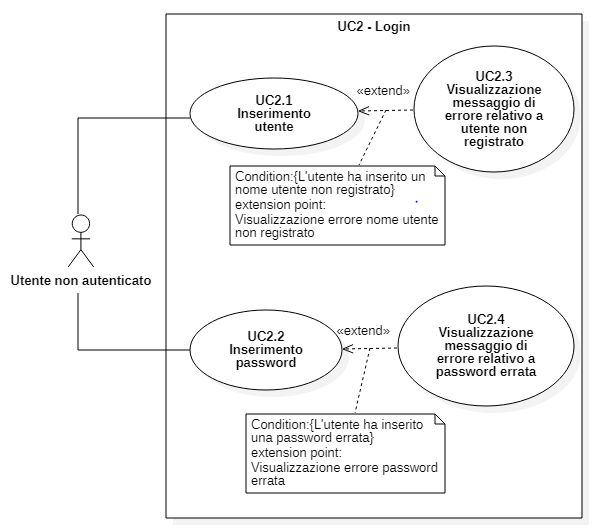
\includegraphics{res/img/caso_duso_login.png}
\subsection{UC2 - Login}
\begin{itemize}
	\item \textbf{Attori Primari:} utente non autenticato;
	\item \textbf{Descrizione:} l'utente tenta di autenticarsi usando le sue credenziali;
	\item \textbf{Scenario principale:} l'utente non è ancora autenticato nella piattaforma ed esegue il login;
	\item \textbf{Pre-condizione:} l'utente non è autenticato nella piattaforma;
	\item \textbf{Post-condizione:} l'utente si autentica con successo, l'utente viene identificato dal sistema nel ruolo di amministratore o operatore. A seconda del ruolo vengono rese disponibili diverse funzionalità.
\end{itemize}

\subsubsection{UC2.1 Inserimento nome utente}
\begin{itemize}
	\item \textbf{Attori Primari:} utente non autenticato;
	\item \textbf{Descrizione:} al fine di potersi autenticare, l'utente è tenuto ad inserire il suo nome utente, campo obbligatorio;
	\item \textbf{Scenario principale:} l'utente inserisce il suo nome utente;
	\item \textbf{Pre-condizione:} il sistema ha reso disponibile il campo per l'inserimento del nome utente;
	\item \textbf{Post-condizione:} l'utente compila il campo con il proprio nome utente.
\end{itemize}	

\subsubsection{UC2.2 Inserimento password}
\begin{itemize}
	\item \textbf{Attori Primari:} utente non autenticato;
	\item \textbf{Descrizione:} al fine di potersi autenticare, l'utente è tenuto ad inserire la sua password, campo obbligatorio;
	\item \textbf{Scenario principale:} l'utente inserisce la sua password;
	\item \textbf{Pre-condizione:} il sistema ha reso disponibile il campo per l'inserimento della password;
	\item \textbf{Post-condizione:} l'utente compila il campo con la propria password.
\end{itemize}	

\subsubsection{UC2.3 Visualizzazione messaggio di errore relativo a utente non registrato}
\begin{itemize}
	\item \textbf{Attori Primari:} utente non autenticato;
	\item \textbf{Descrizione:} l'utente visualizza un messaggio d'errore dovuto al fatto che ha tentato il login con un nome utente non registrato;
	\item \textbf{Scenario principale:} l'utente cerca di fare il login senza essere stato registrato;
	\item \textbf{Pre-condizione:} l'utente cerca di autenticarsi nella piattaforma;
	\item \textbf{Post-condizione:} viene visualizzato un messaggio d'errore per notificare l'utente che un amministratore non ha registrato il suo nome utente nel sistema.
\end{itemize}

\subsubsection{UC2.4 Visualizzazione messaggio di errore relativo a password errata}
\begin{itemize}
	\item \textbf{Attori Primari:} utente non autenticato;
	\item \textbf{Descrizione:} l'utente visualizza un messaggio d'errore dovuto al fatto che ha tentato il login con una password errata;
	\item \textbf{Scenario principale:} l'utente cerca di fare il login con una password sbagliata;
	\item \textbf{Pre-condizione:} l'utente cerca di autenticarsi nella piattaforma;
	\item \textbf{Post-condizione:} viene visualizzato un messaggio d'errore per notificare l'utente ha inserito una password sbagliata.
\end{itemize}

\subsection{UC3 - Logout}
\begin{itemize}
	\item \textbf{Attori Primari:} utente autenticato;
	\item \textbf{Descrizione:} l'utente richiede di eseguire il logout dalla piattaforma. L'utente è quindi tenuto a confermare la procedura di logout;
	\item \textbf{Scenario principale:} l'utente è autenticato alla piattaforma e richiede la procedura di logout tramite l'apposito bottone;
	\item \textbf{Pre-condizione:} l'utente ha eseguito il login e desidera disconnettersi dalla piattaforma;
	\item \textbf{Post-condizione:} Viene eseguita la procedura di logout e l'utente viene notificato con un messaggio.
\end{itemize}


	\newpage
	
	\input{res/casi_duso/sez323_registrazione.tex}
	\newpage
	
	\input{res/casi_duso/sez324_interfaccia.tex}
	\newpage
	



	\newpage

	\section{Requisiti}
	
I requisiti strutturati nel seguente modo:

\begin{itemize}
	
	\item \textbf{codice identificativo:} i codici identificativi sono univoci e conformi alla seguente codifica:
	\begin{center}
		\textbf{R[Priorità]-[Categoria]-[Codice]}
	\end{center}
	dove: 
		\begin{itemize}
			\item \textbf{R:} requisito;
			\item \textbf{Priorità:}
			\begin{itemize}
				\item \textbf{M:} mandatory/obbligatorio, quindi necessario a garantire le funzioni base del prodotto;
				\item \textbf{D:} desirable/desiderabile, cioè non strettamente necessario, ma che porta alla completezza del prodotto;
				\item \textbf{O:} optional/opzionale, quindi che non pregiudica la funzionalità del prodotto finale.
			\end{itemize}
			\item \textbf{Categoria:}
			\begin{itemize}
				\item \textbf{F:} functional/funzionale;
				\item \textbf{P:} performance/prestazionale;
				\item \textbf{Q:} qualitative/qualitativo;
				\item \textbf{C:} constraint/vincolo.
			\end{itemize}
			\item \textbf{Codice:} numero progressivo per riconoscere univocamente il requisito. \\
		\end{itemize}
	\noindent In tabella:
	\item \textbf{Requisito:} il codice identificativo del  requisito;
	\item \textbf{Priorità:} priorità del requisito. Informazione ridondante che però semplifica la lettura;
	
	\item \textbf{Descrizione:} breve ma completa descrizione del requisito, il meno ambigua possibile;
	
	\item \textbf{Fonti:} ogni requisito è derivato da una o più delle seguenti opzioni:
		\begin{itemize}
			\item \glock{capitolato}: requisito individuato in seguito all'analisi del \glock{capitolato};
			\item \textit{interno:} requisito individuato dagli analisti e che si è ritenuto opportuno da aggiungere;
			\item \textit{caso d'uso:} requisito derivato da uno o più casi d'uso. Viene riportato il codice univoco del caso d'uso;
			\item \textit{verbale:} requisiti individuati durante incontri con il proponente.			
		\end{itemize}	
\end{itemize}

\vspace{0.5cm}

\subsection{Requisiti funzionali}

	\newcommand*{\thead}[1]{\multicolumn{1}{c}{\bfseries #1}}	
	\rowcolors{2}{gray!6}{gray!25}
	\setlength{\tabcolsep}{10pt}
	\begin{longtable}[h!] { c c m{8cm} c}
		\caption{Tabella dei requisiti funzionali} \\
		\rowcolor{lightgray}
		\thead{Requisito} & \thead{Priorità} & \thead{Descrizione} & \thead{Fonti} \\ \endhead%
		
		RMF1 & Obbligatorio & Deve essere disponibile per l'utente generico una mappatura dell'ambiente in cui le unità operano & Interno \& UC1 \\
		
		RMF1.1 & Obbligatorio & Deve essere disponibile per l'utente generico una legenda esplicativa della simbologia utilizzata all'interno della mappatura & Interno \& UC1 \\
		
		RMF1.2 & Obbligatorio & La mappatura deve essere aggiornata periodicamente, garantendo che i dati siano coerenti con l'ambiente descritto & Interno \& UC1 \\
		
		RMF1.3 & Obbligatorio & La mappatura deve fornire informazioni sul movimento di unità facenti parte del sistema & Interno \& UC1 \\
		
		RDF1.4 & Desiderabile & La mappatura deve fornire informazioni sul movimento di pedoni presenti nell'ambiente & Interno \& UC1 \\
		
		RMF1.5 & Obbligatorio & La sezione dedicata alla mappatura deve essere sempre disponibile all'utente & Interno \& UC1 \\
		
		RMF2 & Obbligatorio & Un utente può effettuare il login & VE02.5 \& UC2 \\
		
		RMF2.1 & Obbligatorio & Per effettuare login l'utente deve inserire il suo nome utente & VE02.5 \& UC2.1 \\
		
		RMF2.2 & Obbligatorio & Per effettuare login l'utente deve inserire la sua password & VE02.5 \& UC2.2 \\
		
		RMF2.3 & Obbligatorio & Viene visualizzato un errore se viene fornito un nome utente non esistente & VE02.5 \& UC2.3 \\
		
		RMF2.4 & Obbligatorio & Viene visualizzato un errore se se viene fornita una password errata & VE02.5 \& UC2.4 \\
		
		RMF3 & Obbligatorio & Un utente autenticato può effettuare logout & VE02.5 \& UC3 \\
		
		RMF4 & Obbligatorio & Deve essere disponibile una guida utente che contiene le istruzioni operative di utilizzo per un utente autenticato & Interno \& UC4 \\
		
		RMF4.1 & Obbligatorio & La guida utente deve contenere tutte le istruzioni relative alle operazioni elementari che un utente può svolgere all'interno dell'applicativo & Interno \& UC4 \\
		
		RMF4.2 & Obbligatorio & La guida utente deve essere accessibile a tutti e soli gli utenti registrati & Interno \& UC4 \\
		
		RMF5 & Obbligatorio & L'utente autenticato può visualizzare e gestire la lista di unità attive & Capitolato \& UC5 \\
		
		RMF5.1 & Obbligatorio & Ogni elemento della lista di unità fornisce l'ID dell'unità & Interno \& UC5 \\
		
		RMF5.2 & Obbligatorio & Ogni elemento della lista di unità mette a disposizione un ambiente grafico dedicato per visualizzazione e gestione delle proprietà dell'unità & Interno \& UC5 \\
		
		ROF5.2.1 & Opzionale & Dentro all'ambiente grafico dedicato, l'utente autenticato può visualizzare il l'identificativo dell'unità & Interno \& UC5.1.1 \\
		
		RMF5.2.2 & Obbligatorio & L'utente autenticato può visualizzare le coordinate della posizione attuale all'interno della mappa & Interno \& UC5.1.1 \\
		
		RMF5.2.3 & Obbligatorio & L'utente autenticato può visualizzare lo stato dell'unità & Interno \& UC5.1.1 \\
		
		RMF5.2.4 & Obbligatorio & L'utente autenticato può visualizzare la velocità attuale dell'unità & Interno \& UC5.1.1 \\
		
		RMF5.2.5 & Obbligatorio & L'utente autenticato può visualizzare la direzione del prossimo passo suggerita dal sistema & Interno \& UC5.1.1 \\
		
		RMF5.2.6 & Obbligatorio & L'utente autenticato può visualizzare la coda di ordini assegnati all'unità & Interno \& UC5.1.2 \\
		
		RMF5.2.7 & Obbligatorio & L'utente autenticato può impartire il comando \underline{Start} all'unità & Capitolato \& UC5.2.1 \\
		
		RMF5.2.8 & Obbligatorio & L'utente autenticato può impartire il comando \underline{Stop} all'unità & Capitolato \& UC5.2.2 \\
		
		RMF5.2.9 & Obbligatorio & L'utente autenticato può impartire il comando \underline{Go Back} all'unità & Interno \& UC5.2.3 \\
		
		RMF5.2.10 & Obbligatorio & L'utente autenticato può impartire il comando \underline{Shutdown} all'unità & Interno \& UC5.2.4 \\
		
		RMF5.2.11 & Obbligatorio & L'utente autenticato può accodare un nuovo ordine alla lista degli ordini di un'unità & Capitolato \& UC5.2.5 \\
		
		RMF5.2.12 & Obbligatorio & L'utente autenticato può eliminare un ordine dalla lista degli ordini di un'unità qualsiasi sia la sua posizione & Capitolato \& UC5.4.6 \\
		
		RMF6 & Obbligatorio & L'amministratore deve poter visualizzare la lista degli utenti esistenti, e modificarla & VE02.4 \& UC6.1 \\
		
		RMF6.1 & Obbligatorio & L'amministratore deve poter visualizzare il nome utente di ogni utente & Interno \& UC6.1.1 \\
		
		RMF6.2 & Obbligatorio & L'amministratore deve poter visualizzare la password di ogni utente & Interno \& UC6.1.1 \\
		
		RMF6.3 & Obbligatorio & L'amministratore deve poter creare nuovi utenti & VE02.4 \& UC6.1.3 \\
		
		RMF6.3.1 & Obbligatorio & La creazione di un nuovo utente richiede l'input delle credenziali per il nuovo utente & VE02.4 \& UC6.1.6 \\
		
		RMF6.4 & Obbligatorio & L'amministratore deve poter modificare utenti esistenti & VE02.4 \& UC6.1.4 \\
		
		RMF6.4.1 & Obbligatorio & La modifica di un utente esistente richiede l'input delle credenziali per l'utente & VE02.4 \& UC6.1.6 \\
		
		RMF6.5 & Obbligatorio & L'amministratore deve poter eliminare utenti esistenti & VE02.4 \& UC6.1.5 \\
		
		RMF6.6 & Obbligatorio & L'input delle credenziali utente richiede un nome utente & VE02.4 \& UC6.1.7 \\
		
		RMF6.7 & Obbligatorio & L'input delle credenziali utente richiede una password & VE02.4 \& UC6.1.8 \\
		
		RMF6.8 & Obbligatorio & L'input delle credenziali utente richiede lo status & VE02.4 \& UC6.1.9 \\
		
		RMF6.9 & Obbligatorio & Viene visualizzato un errore se è stato fornito un nome utente già assegnato ad un utente esistente & VE02.4 \& UC6.1.10 \\
		
		RMF6.10 & Obbligatorio & Viene visualizzato un errore se viene fornita una password non formattata correttamente & VE02.4 \& UC6.1.11 \\
		
		RMF7 & Obbligatorio & L'amministratore deve poter modificare la mappa formattandola opportunamente & Capitolato \& UC6.2.2 \\
		
		RMF7.1 & Obbligatorio & Viene visualizzato un errore se si tenta di formattare la mappa erratamente & Capitolato \& UC6.2.3 \\
		
		RMF8 & Obbligatorio & L'amministratore deve poter visualizzare la lista unità gestite dal sistema, e modificarla & VE02.4 \& UC6.3 \\
		
		RMF8.1 & Obbligatorio & L'amministratore deve poter visualizzare l'ID di ogni unità & Interno \& UC6.3.1 \\
		
		RMF8.2 & Obbligatorio & L'amministratore deve poter creare nuove unità & VE02.4 \& UC6.3.3 \\
		
		RMF8.2.1 & Obbligatorio & La creazione di una nuova unità, da parte dell'amministratore, richiede l'input del rispettivo ID & VE02.4 \& UC6.3.6 \\
		
		RMF8.3 & Obbligatorio & L'amministratore deve poter modificare unità esistenti & VE02.4 \& UC6.3.4 \\
		
		RMF8.3.1 & Obbligatorio & La modifica di un'unità esistente, da parte dell'amministratore, richiede l'input  del rispettivo ID & VE02.4 \& UC6.3.6 \\
		
		RMF8.4 & Obbligatorio & L'amministratore deve poter eliminare unità esistenti & VE02.4 \& UC6.3.5 \\
		
		RMF8.5 & Obbligatorio & Viene visualizzato un errore se viene fornito un ID già assegnato ad un'unità esistente & VE02.4 \& UC6.3.7 \\
		
		RMF9 & Obbligatorio & L'unità, dotata di sensoristica, deve comunicare al sistema la posizione relativa degli ostacoli che riescono a rilevare & VE02.6 \\
		
		RMF10 & Obbligatorio & L'unità comunica in \glock{real-time} al sistema le proprie coordinate & Capitolato \\
		
		RMF11 & Obbligatorio & All'unità viene assegnato dal sistema un percorso definito per poter raggiungere il prossimo \glock{POI} & Capitolato \\
		
		RMF12 & Obbligatorio & L'unità dispone di una coda degli ordini con i prossimi \glock{POI} da raggiungere & Capitolato \\
		
		RMF13 & Obbligatorio & L'unità riceve modifiche alla coda degli ordini solo quando si trova alla base di ricarica & Interno \& UC5 \\
		
		RMF14 & Obbligatorio & L'unità con coda degli ordini vuota ritorna alla base & Interno \& UC5 \\
		
		RMF15 & Obbligatorio & L'unità dispone di una velocità massima & Capitolato \\
		
		RMF16 & Obbligatorio & L'unità può assumere lo stato \underline{Going to X} & Interno \& UC5 \\
		
		RMF17 & Obbligatorio & L'unità può assumere lo stato \underline{Stop} & Interno \& UC5 \\
		
		RMF18 & Obbligatorio & L'unità può assumere lo stato \underline{Base} & Interno \& UC5 \\
		
		RMF19 & Obbligatorio & L'unità può assumere lo stato \underline{Error Y} & Interno \& UC5 \\
		
		RMF20 & Obbligatorio & Il sistema dispone di un algoritmo per il calcolo del percorso che l'unità deve effettuare per raggiungere il prossimo \glock{POI} & Capitolato \\
		
		RMF20.1 & Obbligatorio & L'algoritmo di calcolo del percorso deve evitare la collisione delle unità con ostacoli & Capitolato \\
		
		RMF20.2 & Obbligatorio & L'algoritmo di calcolo del percorso deve evitare la collisione delle unità con altre unità & Capitolato \\
		
		ROF20.3 & Opzionale & L'algoritmo di calcolo del percorso deve restituire il percorso ottimo & Capitolato \\
		
		RDF21 & Desiderabile & Nella mappa sono presenti dei pedoni & Capitolato \\
		
		RDF21.1 & Desiderabile & Il pedone comunica in \glock{real-time} al sistema la propria posizione & VE02.8 \\
		
		RDF21.2 & Desiderabile & Il pedone rappresenta un ostacolo mobile per l'unità & Capitolato \\

	\end{longtable}

\newpage

\subsection{Requisiti di vincolo}

\rowcolors{2}{gray!6}{gray!25}
\setlength{\tabcolsep}{10pt}
\begin{longtable}[h!] { c c m{8.5cm} c}
	\caption{Tabella dei requisiti di vincolo} \\
	\rowcolor{lightgray}
	\thead{Requisito} & \thead{Priorità} & \thead{Descrizione} & \thead{Fonti} \\ \endhead%
	
	RMC1 & Obbligatorio & Ogni entità sviluppata facente parte del sistema dovrà essere contenuta in un container \glock{Docker} del quale andrà fornito il \glock{Dockerfile} & Capitolato \\
	
	RMC1.1 & Obbligatorio & Deve essere fornito un \glock{Dockerfile} con il motore di calcolo & Capitolato \\
	
	RMC1.2 & Obbligatorio & Deve essere fornito un \glock{Dockerfile} con il visualizzatore \glock{real-time} & Capitolato \\
	
	RMC1.3 & Obbligatorio & Deve essere fornito un \glock{Dockerfile} per la singola unità & Capitolato \\
	
	RDC1.4 & Desiderabile & Deve essere fornito un \glock{Dockerfile} per il singolo pedone & Capitolato \\
	
\end{longtable}

\newpage

\subsection{Requisiti di qualità}

\rowcolors{2}{gray!6}{gray!25}
\setlength{\tabcolsep}{10pt}
\begin{longtable}[h!] { c c m{8.5cm} c}
	\caption{Tabella dei requisiti di qualità} \\
	\rowcolor{lightgray}
	\thead{Requisito} & \thead{Priorità} & \thead{Descrizione} & \thead{Fonti} \\ \endhead%
	
	RMQ1 & Obbligatorio & Il prodotto va rilasciato con la licenza \glock{open-source} più aperta possibile in base alle librerie utilizzate & VE01.4 \\
	
	RMQ2 & Obbligatorio & Il prodotto deve essere conforme con quanto dichiarato nel documento \dext{Piano di Qualifica v1.0.0} e successivi aggiornamenti del medesimo & Interno \\
	
	RMQ3 & Obbligatorio & Devono essere realizzati test di unità e di integrazione per verificare le singole componenti del prodotto & Interno \\
	
\end{longtable}

\vspace{3cm}

\subsection{Requisiti prestazionali}
	
\rowcolors{2}{gray!6}{gray!25}
\setlength{\tabcolsep}{10pt}
\begin{longtable}[h!] { c c m{8.5cm} c }
	\caption{Tabella dei requisiti prestazionali} \\
	\rowcolor{lightgray}
	\thead{Requisito} & \thead{Priorità} & \thead{Descrizione} & \thead{Fonti} \\ \endhead%
	
	RMP1 & Obbligatorio & Il tempo di aggiornamento della mappatura rispetto alla posizione delle unità nell'ambiente deve essere $\leq$ 5 secondi & Interno \& VE01.2 \\ 
	
	RDP1.1 & Desiderabile & Il tempo di aggiornamento della mappatura rispetto alla posizione delle unità nell'ambiente deve essere $\leq$ 2.5 secondi & Interno \& VE01.2 \\
	
	ROP1.2 & Opzionale & Il tempo di aggiornamento della mappatura rispetto alla posizione delle unità nell'ambiente deve essere $\leq$ 1 secondi & Interno \& VE01.2 \\
	
	RMP2 & Obbligatorio & Il servizio non deve mai essere interrotto secondo una logica di \glock{zero downtime} & Capitolato \\
	
\end{longtable}

\newpage

\subsection{Tracciamento}

\subsubsection{Fonte - Requisiti}

\rowcolors{2}{gray!6}{gray!25}
\setlength{\tabcolsep}{10pt}
\begin{longtable}[h!] { >{\centering}m{5cm} >{\centering}m{5cm} }
	\caption{Tabella di tracciamento fonte-requisiti} \\
	\rowcolor{lightgray}
	\thead{Fonte} & \thead{Requisiti} \\ \endhead%
	
	Capitolato & RMF5 \\
	 RMF5.2.7 \\
	 RMF5.2.8 \\
	 RMF5.2.11 \\
	 RMF5.2.12 \\
	 RMF7 \\
	 RMF7.1 \\
	 RMF10 \\
	 RMF11 \\
	 RMF12 \\
	 RMF15 \\
	 RMF20 \\
	 RMF20.1 \\
	 RMF20.2 \\
	 ROF20.3 \\
	 RDF21 \\
	 RDF21.2 \\
	 RMP2 \\
	 RMC1 \\
	 RMC1.1 \\
	 RMC1.2 \\
	 RMC1.3 \\
	 RDC1.4
	 \tabularnewline
	 Interno & RMF1 \\
	 RMF1.1 \\
	 RMF1.2 \\
	 RMF1.3 \\
	 RDF1.4 \\
	 RMF1.5 \\
	 RMF4 \\
	 RMF4.1 \\
	 RMF4.2 \\
	 RMF5.1 \\
	 RMF5.2 \\
	 ROF5.2.1 \\
	 RMF5.2.2 \\
	 RMF5.2.3 \\
	 RMF5.2.4 
	 \tabularnewline
	 %Qua bisogna fixare 
	 Interno & RMF5.2.5 \\ 
	 RMF5.2.6 \\
	 RMF5.2.9 \\
	 RMF5.2.10 \\
	 RMF6.1 \\
	 RMF6.2 \\
	 RMF8.1 \\
	 RMF13 \\
	 RMF14 \\ 
	 RMF16 \\
	 RMF17 \\
	 RMF18 \\
	 RMF19 \\
	 RMP1 \\
	 RDP1.1 \\
	 ROP1.2 \\
	 RMQ2 \\
	 RMQ3 
	 \tabularnewline
	 UC1 & RMF1 \\
	 RMF1.1 \\
	 RMF1.2 \\
	 RMF1.3 \\
	 RDF1.4 \\
	 RMF1.5 
	 \tabularnewline
	 UC2 & RMF2 
	 \tabularnewline
	  UC2.1 & RMF2.1
	 \tabularnewline
	  UC2.2 & RMF2.1 
	 \tabularnewline
	  UC2.3 & RMF2.3 
	 \tabularnewline
	  UC2.4 & RMF2.4 
	 \tabularnewline
	  UC3 & RMF3 
	 \tabularnewline
	  UC4 & RMF4\\
	  RMF4.1 \\
	  RMF4.2
	 \tabularnewline
	 UC5 & RMF5 \\
	 RMF5.1 \\
	 RMF5.2 \\
	 RMF13 \\
	 RMF14 \\
	 RMF16 \\
	 RMF17 \\
	 RMF18 \\
	 RMF19 
	 \tabularnewline
	 UC5.1 & ROF5.2.1 \\
	 RMF5.2.2 \\
	 RMF5.2.3 \\
	 RMF5.2.4 \\
	 RMF5.2.5 
	 \tabularnewline
	 UC5.1.2 & RMF5.2.6 
	 \tabularnewline
	 UC5.2.1 & RMF5.2.7 
	 \tabularnewline
	 UC5.2.2 & RMF5.2.8 
	 \tabularnewline
	 UC5.2.3 & RMF5.2.9 
	 \tabularnewline
	 UC5.2.4 & RMF5.2.10 
	 \tabularnewline
	 UC5.2.5 & RMF5.2.11 
	 \tabularnewline
	 UC5.4.6 & RMF5.2.12 
	 \tabularnewline
	 UC6.1 & RMF6
	 \tabularnewline
	 UC6.1.1 & RMF6.1 \\ 
	 RMF6.2
	 \tabularnewline
	 UC6.1.3 & RMF6.3
	 \tabularnewline
	 UC6.1.4 & RMF6.4
	 \tabularnewline
	 UC6.1.5 & RMF6.5
	 \tabularnewline
	 UC6.1.6 & RMF6.3.1 \\ 
	 RMF6.4.1
	 \tabularnewline
	 UC6.1.7 & RMF6.6
	 \tabularnewline
	 UC6.1.8 & RMF6.7
	 \tabularnewline
	 UC6.1.9 & RMF6.8
	 \tabularnewline
	 UC6.1.10 & RMF6.9
	 \tabularnewline
	 UC6.1.11 & RMF6.10
	 \tabularnewline
	 UC6.2.2 & RMF7
	 \tabularnewline
	 UC6.2.3 & RMF7.1
	 \tabularnewline
	 UC6.3 & RMF8
	 \tabularnewline
	 UC6.3.1 & RMF8.1
	 \tabularnewline
	 UC6.3.3 & RMF8.2
	 \tabularnewline
	 UC6.3.4 & RMF8.3
	 \tabularnewline
	 UC6.3.5 & RMF8.4
	 \tabularnewline
	 UC6.3.6 & RMF8.2.1 \\ 
	 RMF8.3.1 
	 \tabularnewline
	 UC6.3.7 & RMF8.5
	 \tabularnewline
	 VE01.2 & RMP1 \\
	 RDP1.1 \\
	 ROP1.2 
	 \tabularnewline
	 VE01.4 & RMQ1
	 \tabularnewline
	 VE02.4 & RMF6\\
	 RMF6.3 \\
	 RMF6.3.1 \\
	 RMF6.4 \\
	 RMF6.4.1 \\
	 RMF6.5 \\
	 RMF6.6 \\
	 RMF6.7 \\
	 RMF6.8 \\
	 RMF6.9 \\
	 RMF6.10 
	 \tabularnewline
	 VE02.5 & RMF2 \\
	 RMF2.1 \\
	 RMF2.2 \\
	 RMF2.3 \\
	 RMF2.4 \\
	 RMF3
	 \tabularnewline
	 VE02.8 & RDF21.1
	 \tabularnewline
	
\end{longtable}

\newpage

\subsubsection{Requisito - Fonti}

\rowcolors{2}{gray!6}{gray!25}
\setlength{\tabcolsep}{10pt}
\begin{longtable}[h!] { >{\centering}m{5cm} >{\centering}m{5cm} }
	\caption{Tabella di tracciamento requisito-fonti} \\
	\rowcolor{lightgray}
	\thead{Requisito} & \thead{Fonti} \\ \endhead%
	
	RMF1    &  Interno\\UC1
	\tabularnewline
	RMF1.1  & Interno \\UC1
	\tabularnewline
	RMF1.2  & Interno\\UC1
	\tabularnewline
	RMF1.3   & Interno\\UC1
	\tabularnewline
	RDF1.4 & Interno\\UC1
	\tabularnewline
	RMF1.5 & Intern\\UC1
	\tabularnewline
	RMF2 & VE02.5\\UC2
	\tabularnewline
	RMF2.1 & VE02.5\\UC2.1
	\tabularnewline
	RMF2.2 & VE02.5\\UC2.2
	\tabularnewline
	RMF2.3 & VE02.5\\UC2.3
	\tabularnewline
	RMF2.4 & VE02.5\\UC2.4
	\tabularnewline
	RMF3 & VE02.5\\UC3
	\tabularnewline
	RMF4 & Interno\\UC4
	\tabularnewline
	RMF4.1 & Interno\\UC4
	\tabularnewline
	RMF4.2 & Interno\\UC4
	\tabularnewline
	RMF5 & Capitolato\\UC5
	\tabularnewline
	RMF5.1 & Interno\\UC5
	\tabularnewline
	RMF5.2 & Interno\\UC5
	\tabularnewline
	ROF5.2.1 &  Interno\\UC5.1.1
	\tabularnewline
	RMF5.2.2 & Interno\\UC5.1.1
	\tabularnewline
	RMF5.2.3 & Interno\\UC5.1.1
	\tabularnewline
	RMF5.2.4 & Interno\\UC5.1.1
	\tabularnewline
	RMF5.2.5 & Interno\\UC5.1.1
	\tabularnewline
	RMF5.2.6 & Interno\\UC5.1.2
	\tabularnewline
	RMF5.2.7 &  Capitolato\\UC5.2.1
	\tabularnewline
	RMF5.2.8 & Capitolato\\UC5.2.2
	\tabularnewline
	RMF5.2.9 & Interno\\UC5.2.3
	\tabularnewline
	RMF5.2.10 & Interno\\UC5.2.4
	\tabularnewline
	RMF5.2.11 & Capitolato\\UC5.2.5
	\tabularnewline
	RMF5.2.12 & Capitolato\\UC5.4.6
	\tabularnewline
	RMF6 & VE02.4\\UC6.1
	\tabularnewline
	RMF6.1 & Interno\\UC6.1.1
	\tabularnewline
	RMF6.2 & Interno\\UC6.1.1
	\tabularnewline
	RMF6.3 & VE02.4\\UC6.1.3
	\tabularnewline
	RMF6.3.1 & VE02.4\\UC6.1.6
	\tabularnewline
	RMF6.4 & VE02.4\\UC6.1.4
	\tabularnewline
	RMF6.4.1 & VE02.4\\UC6.1.6
	\tabularnewline
	RMF6.5 & VE02.4\\UC6.1.5
	\tabularnewline
	RMF6.6 & VE02.4\\UC6.1.7
	\tabularnewline
	RMF6.7 & VE02.4\\UC6.1.8
	\tabularnewline
	RMF6.8 & VE02.4\\UC6.1.9
	\tabularnewline
	RMF6.9 & VE02.4\\UC6.1.10
	\tabularnewline
	RMF6.10 & VE02.4\\UC6.1.11
	\tabularnewline
	RMF7 & Capitolato\\UC6.2.2
	\tabularnewline
	RMF7.1 & Capitolato\\UC6.2.3
	\tabularnewline
	RMF8 & VE02.4\\UC6.3
	\tabularnewline
	RMF8.1  & Interno\\UC6.3.1
	\tabularnewline
	RMF8.2 & VE02.4\\UC6.3.3
	\tabularnewline
	RMF8.2.1  & VE02.4\\UC6.3.6
	\tabularnewline
	RMF8.3 & VE02.4\\UC6.3.4
	\tabularnewline
	RMF8.3.1 & VE02.4\\UC6.3.6
	\tabularnewline
	RMF8.4 & VE02.4\\UC6.3.5
	\tabularnewline
	RMF8.5 & VE02.4\\UC6.3.7
	\tabularnewline
	RMF9 & VE02.6
	\tabularnewline
	RMF10 & Capitolato
	\tabularnewline
	RMF11 & Capitolato
	\tabularnewline
	RMF12 & Capitolato
	\tabularnewline
	RMF13 & Interno\\UC5
	\tabularnewline
	RMF14 & Interno\\UC5
	\tabularnewline
	RMF15 & Capitolato
	\tabularnewline
	RMF16 & Interno\\UC5
	\tabularnewline
	RMF17 & Interno\\UC5
	\tabularnewline
	RMF18 & Interno\\UC5
	\tabularnewline
	RMF19 & Interno\\UC5
	\tabularnewline
	RMF20 & Capitolato
	\tabularnewline
	RMF20.1 & Capitolato
	\tabularnewline
	RMF20.2 & Capitolato
	\tabularnewline
	ROF20.3 & Capitolato
	\tabularnewline
	RDF21 & Capitolato
	\tabularnewline
	RDF21.1 & VE02.8
	\tabularnewline
	RDF21.2 & Capitolato
	\tabularnewline
	RMP1 & Interno\\VE01.2
	\tabularnewline
	RDP1.1 & Interno\\VE01.2
	\tabularnewline
	ROP1.2 & Interno\\VE01.2
	\tabularnewline
	RMP2 & Capitolato
	\tabularnewline
	RMQ1 & VE01.4
	\tabularnewline
	RMQ2 & Interno
	\tabularnewline
	RMQ3 & Interno
	\tabularnewline
	RMC1 & Capitolato
	\tabularnewline
	RMC1.1 & Capitolato
	\tabularnewline
	RMC1.2 & Capitolato
	\tabularnewline
	RMC1.3 & Capitolato
	\tabularnewline
	RDC1.4 & Capitolato
	\tabularnewline
	
\end{longtable}


	\newpage

\end{document}